\documentclass[12pt]{article}

\usepackage{fullpage} %
\usepackage{xspace} %
\usepackage{color} %
\usepackage{graphicx} %
\usepackage{amsmath} %
\usepackage{amssymb}
\usepackage{paralist}%
\usepackage{hyperref}
\usepackage{physics}
\usepackage{qcircuit}
\usepackage{multirow}
\usepackage{algorithm}
\usepackage[noend]{algpseudocode}
\usepackage{amsthm}
\usepackage{listings}

\renewcommand\H{\mathcal{H}}
\newcommand\bmat[1]{\begin{bmatrix} #1 \end{bmatrix}}
\newcommand\K[1]{\ket{#1}}
\definecolor{c}{rgb}{0.0, 0.44, 1.0}
%\newcommand{\edgee}[1]{\begin{math}\stackrel{#1}{\longrightarrow}\end{math}}

\newcounter{problem}
\newcommand{\problem}[1]{\stepcounter{problem}
  \noindent{\bf Problem \theproblem: }#1\\[1pc]}
\parindent=0pt
\setlength{\parskip}{1pc}

\newcounter{task}
\newcommand{\task}[1]{\stepcounter{task}
  \noindent{\bf Task \thetask: }#1\\[1pc]}
\parindent=0pt
\setlength{\parskip}{1pc}


\begin{document}
\begin{center}
\Large\bf How Pheromone Trails Effect Navigation within an Ant Colony\\[1pc]
\large\bf By: Natalie Tobiason
\end{center}

\section{Equations}
\begin{enumerate}
  \item ant navigation when no pheromone present
  \item probability ant follows pheromone trail (home trail 99\%, food trail 80-ish\%)
  \item pheromone concentration depletion $$ C_i[k+1]=C_i[k](\kappa) $$
  \item the ability of ants to detect and respond to pheromone $$ f(C) = \bigg( 1+ \frac{C}{1+\rho C}\bigg)^\zeta$$
\end{enumerate}

\section{Variables}
\begin{enumerate}
  \item $C(x,y)$ pheremone concentration at $(x,y)$
  \item ants emit pheromone at given rate $\eta = 0.07$
  \item pheromone evaporates at rate $\kappa = 0.015$
  \item the mean density of ants $\rho_0$. (number of ants present)
  \item average pheromonal field $\sigma_0 = \rho_0\eta/\kappa$
  \item ordered behavior (non-random walk) sets in when $\sigma_0 f'(\sigma_0)/f(\sigma_0)-1/\beta > 0$
\end{enumerate}

\section{Modelling foraging ants in a dynamic and confined environemtn}
https://www-sciencedirect-com.colorado.idm.oclc.org/science/article/pii/S030326471000239X?via\%3Dihub
\\ \textbf{Notes:}
\begin{itemize}
  \item half life of pheremone on plastic is about nine minutes and about 3 minutes on paper
\end{itemize}

% 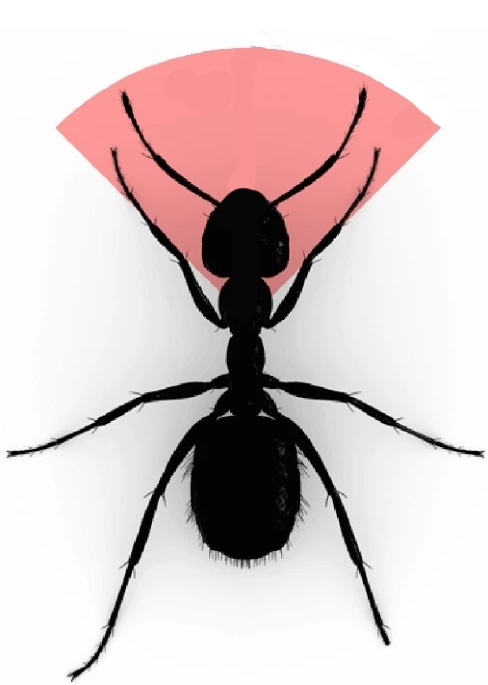
\includegraphics[scale=0.5]{/Users/nattobiason/Projects/GameDev/HelloSDL/img/ant_vision.jpg}

\section{Random Walk}

$ \theta = \pi /3 $ \\
$ \text{CRW theta }= \pi /2 $ \\

$$ \triangle X_{i+1} = v\big[ \text{ cos}(\theta_i+\theta_i^{\text{CRW}}) \big] $$
$$ \triangle Y_{i+1} = v\big[ \text{ sin}(\theta_i+\theta_i^{\text{CRW}}) \big] $$


\section{Biased Random Walk}

$ w = ? $ \\
$ \theta = \pi /3 $ \\
$ \text{CRW theta }= \pi /2 $ \\
$ \text{BRW theta }= \pi /3 $ \\
$ \theta_0 \in [\frac{2\pi}{3}, \frac{\pi}{2}, \frac{\pi}{3}] $ 

$$ \triangle X_{i+1} = v\big[ w \text{cos}(\theta_0+\theta_i^{\text{BRW}}) + (1-w) \text{cos}(\theta_i+\theta_i^{\text{CRW}}) \big] $$
$$ \triangle Y_{i+1} = v\big[ w \text{sin}(\theta_0+\theta_i^{\text{BRW}}) + (1-w) \text{sin}(\theta_i+\theta_i^{\text{CRW}}) \big] $$

$\beta = \pi / 3 $ \\
$ \varphi = \text{ ant height} $

\vskip0.5pc

Area of Ant $ = x^2 + y^2 \leq \Big( \frac{\text{ant height}}{2}\Big)^2$ (in our case, the ant is 10x10 pixels so) \\
$\hspace*{2.5cm} = x^2+y^2 \leq 25 $\\

  $$\text{Sensing area}$$

$$  2\int_{-\frac3{\pi}y}^{\frac3{\pi}y} \sqrt{-x^2+100}-\sqrt{-x^2-25} \,dx $$

$$ \text{where } (x, y) \text{ is the current position of the ant} $$

$ y = \sqrt{-x^2+100}$\\

$y = \frac{\pi}{3}x$\\

$y = -\frac{\pi}{3}x$

\newpage
\begin{lstlisting}
  if pheremone present
    
    if max(pheremone_concentration) == A
      biased_random_walk(bias = 2pi/3)

    else if max(pheremone_concentration) == B
      biased_random_walk(bias = pi/2)

    else if max(pheremone_concentration) == C
      biased_random_walk(bias = pi/3)

  
\end{lstlisting}

\end{document}